\section{Current market}

The process of humanitarian demining consists mainly of three aspects, firstly to prepare the terrain or mine-affected area. This includes removing objects and clearing of vegetation, which is mostly done by heavily armoured vehicles. That process usually triggers some of the mines but not all. Secondly is to precisely locate the mine and thirdly to remove or destroy it \cite{HiddenKillers2019}.

New technology should try to help in one of these areas. Multiple methods for demining have been developed since the introduction of landmines in warfare. These methods vary from, training and using animals for mine localization, to using advanced technology for localization and demining. Regarding this, advanced technologies are in use, these are however mostly reserved for the military \cite{HiddenKillers2019}.
The process of military demining is in some ways like humanitarian demining. However, it is different in the way, that the goal is not to clear the minefields and make them safe for civilian use, but to make a safe passage through the minefields \cite{HiddenKillers2019}. A comparison between these, military and humanitarian demining, can be seen in Figure \ref{fig:military_humanitarian_demining}.

\medskip

\begin{figure}[h]
  \centering
      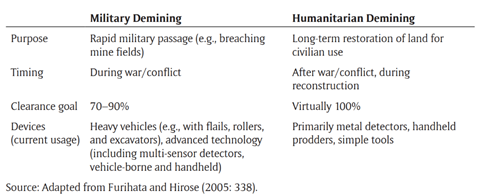
\includegraphics[width=1\textwidth]{00 - Images/military_humanitarian_demining.png}
  \caption{Comparison of Military and Humanitarian Demining \cite{HiddenKillers2019}}
  \label{fig:military_humanitarian_demining}
\end{figure}

In military demining-operations, armoured machines or vehicles are often used since they activate the mines and hereby destroy them. Nevertheless, these vehicles have shown to be ineffective in difficult terrain and are mostly reserved for the military \cite{6LeggedRobot2007}. Even though advancements in technology are being made, they still need more development, testing, and a cost reduction, before they can be properly implemented by humanitarian workers \cite{HiddenKillers2019}. 

\subsection{Manual demining methods}

\subsubsection*{metal detectors}

a metal detector i used to measures disturbances in magnetic fields caused by metal objects in the ground. the problem with this is that it is a very slow process.

\subsubsection*{mine prodding}
Mine prodding Which is accomplished by using some form of prodding tool a trowel, bayonet or something of similar length and sharpness. When mine prodding the goal is to ascertain the location of a mine that has previously been located by a metal detector. The prod is inserted in the dirt at around a 30 degree angle and it is then pushed into the ground with the goal of hitting the mine at an angel so as to avoid the triggering mechanism. Mine prodding is only used in the excavating of mines that have been found using a metal detector or similar method in humanitarian demining as it is considered to be to dangerous to use for locating mines.

\subsubsection*{animals in demining}
Attempts to use animals to locate mines have proven somewhat use full; A example of this dogs and rats have been used for locating mines. Dogs have proven somewhat use full in this regard as they can be trained to sniff out the explosives. The problem with using dogs for locating mines is that the dogs get often get confused if there is more than one source of the smell they are trying to locate \cite{DeminingDogs2016}. Rats can be trained for this as well but have not had this problem\cite{PouchedRats2016}. Another problem in the use of animals is that you can not be as methodical in your search as you might like.

\subsubsection*{visual inspection}
Locating a mine using visual detection. Is as the name implies to attempt to locate mines using vision. While the accuracy of a visual inspection can be improved with knowledge of mines and methods of hiding them it is still not a very trustworthy method for locating\cite{LandmineDetection2000}.

\begin{figure} [H]
    \centering
    \begin{subfigure}[b]{0.28\textwidth}
        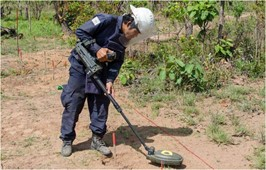
\includegraphics[width=\textwidth]{00 - Images/man_with_detector.jpg}
        \caption{Finding landmines with metal detector \cite{ManDetector2018}}
        \label{fig:man_with_detector}
    \end{subfigure}
    ~ %add desired spacing between images, e. g. ~, \quad, \qquad, \hfill etc. 
      %(or a blank line to force the subfigure onto a new line)
    \begin{subfigure}[b]{0.28\textwidth}
        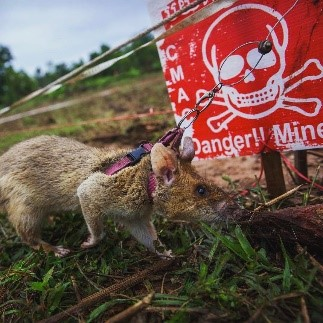
\includegraphics[width=\textwidth]{00 - Images/rat_finding_mines.jpg}
        \caption{Rats sniffing out bombs}
        \label{fig:rat_finding_mines}
    \end{subfigure}
    ~ %add desired spacing between images, e. g. ~, \quad, \qquad, \hfill etc. 
    %(or a blank line to force the subfigure onto a new line)
    \begin{subfigure}[b]{0.28\textwidth}
        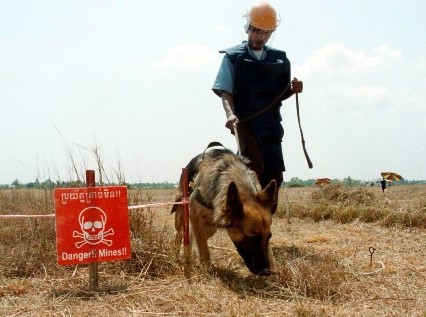
\includegraphics[width=\textwidth]{00 - Images/dog_finding_mines.jpg}
        \caption{Dogs sniffing out landmines}
        \label{fig:dog_finding_mines}
    \end{subfigure}
    %\caption{Pictures of animals}\label{fig:animals}
\end{figure}

It becomes very clear that advancements and innovations in humanitarian demining should be made. Robots could be a huge help in demining an area since they potentially eliminate the human risk associated with detecting landmines. Multiple demining robots have already been made with the intent of finding and/or disposing landmines and unexploded ordinance. These robots each work very differently and use different technology to detect landmines all to make the demining process easier, faster, and safer \cite{MotionPlanningRobot2011}.

\subsection{Current Demining Robots}

In general, modern humanitarian ground-based demining robots can be divided into three categories, based on movement types.
\begin{itemize}
\setlength{\itemsep}{0.05\baselineskip}
	\item Continuous track robots
	\item Wheeled robots
	\item Legged robots
\end{itemize}

Each of these types has its strengths and weaknesses. Where continuous tracked and wheeled robots provide easy accessibility, since most of the parts required for construction can be found in local existing technologies, their contact to the ground is high, which increases the risk of accidentally triggering a mine. Opposite to this, the legged robots have a smaller contact area with the ground and therefore run with a smaller risk of triggering. On top of this, legged robots provide omnidirectional movement, i.e. it can change directions while not needing to make a turn, ex. going in one direction, stopping, continue in 27 degrees left from the previous direction. This derivatively decreases the risk of accidental triggers even more \cite{6LeggedRobot2007}. However, we assume these robots require more advanced mechanical systems, which increases cost, and the need for specialized parts that are less likely to be found in the local area where the demining takes place. Wheels can be made omnidirectional as well, but that solution is not suitable for rough terrain, due to various places that dirt can get stuck.\\

It is our opinion that the tracked and wheeled solutions outweigh the legged robots in the current market, mainly for their simplicity in both construction, system, and operator requirements. Furthermore, we assume that wheels are cheaper than tracks, due to fewer parts, needed to construct a wheel, than a track. Therefore, we want to work with a wheeled robot.

\newpage

Humanitarian demining robots can likewise be divided into 3 categories based on autonomy, as such:
\begin{itemize}
\setlength{\itemsep}{0.05\baselineskip}
	\item Fully operator-controlled robots
	\item Semi-autonomous robots
	\item Fully autonomous robots
\end{itemize}

A fully operator-controlled robot can have a simple design. But these robots require a highly qualified/trained operator, to make full use of the robot. We assume that these operators are hard to come by in the local area, this can be thought of as an issue for these types of robots.\\

Moving up the categories to more autonomous solutions, would, of course, be a more ideal solution because this would decrease human error and the human risk factor, i.e. operator will not be close to a possible explosion. However, this, as with anything else, comes with higher expenses and without further improvements on the robots, to lower the expenses it could be difficult to make them it more affordable \cite{6LeggedRobot2007}. Although we assess that a fully autonomous solution will be cheaper in the long run, based on operating expenses. Therefore, we prefer a fully autonomous solution.

\subsection{Sensors}

We already provided information on less advanced methods for mine detection, see ‘Primitive demining methods’, however more advanced technology such as the use of detection sensors could provide a safer alternative. These sensors can be divided into the following groups \cite{HumanitarianDemining2017}:
\begin{itemize}
\setlength{\itemsep}{0.05\baselineskip}
	\item Explosive detectors
	\item Electromagnetic sensors
	\item Electro-optic sensors
\end{itemize}

Explosive detectors are used to detect the explosive material of a mine. Electromagnetic sensors, such as metal detectors (MD), which are used to measure magnetized metals, or ground penetrating radar (GPR), which can identify plastic. An electro-optic sensor such as an infrared sensor (IR), uses light waves to measure the distance to some objects in the soil. All these could potentially be used to locate mines \cite{HumanitarianDemining2017}.

Limitations on these sensors do exist, which is why a combination of multiple sensors might be the best option for a mine detection robot. For instance, an electro-optic sensor such as an infrared sensor cannot be used to centre specific mines. This means they are only capable of scanning an area. Ground-penetrating radar is relying on the ground condition to determine the depth of its ground penetration but can however detect other materials than metal beneath the ground. Metal detectors might be cheap and reliable but can, as the name implies, only detect metal \cite{HumanitarianDemining2017}.
So in general, making a robot effective, means using a few different sensors and detectors to cover the limitations of the single one \cite{6LeggedRobot2007}.

\subsection{Current Humanitarian Demining Robots}

Since humanitarian demining still heavily relies on dangerous primitive techniques, a lot of re-search is being done with the intent of creating a viable robot to be used in humanitarian demining. Figure \ref{fig:field_robots_for_humanitarian_demining_2014} shows a table, which is taken from \cite{FieldRobots2014}. It presents six modern-day field robots with different specifications, all of which have been presented as a possible solution to the demining problem \cite{FieldRobots2014}.

\begin{figure}[ht]
  \centering
      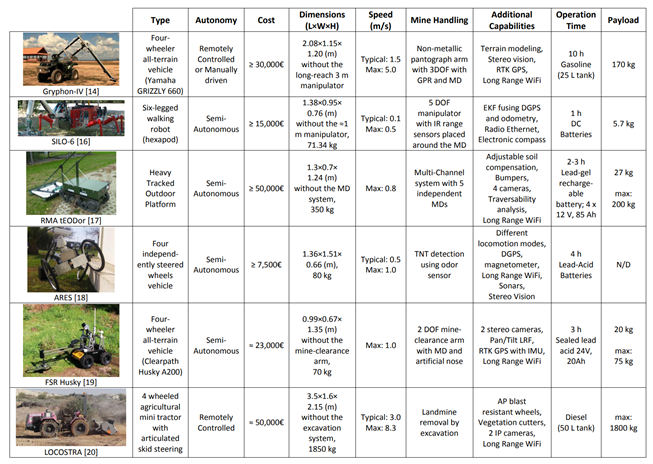
\includegraphics[width=1\textwidth]{00 - Images/field_robots_for_humanitarian_demining_2014.png}
  \caption{Deploying field robots for humanitarian demining: Challenges, requirements, and research trends, 2014 \cite{FieldRobots2014}}
  \label{fig:field_robots_for_humanitarian_demining_2014}
\end{figure} \todo{This cut out table is quite crap, we should make something thats relevant for this project \#notflaming}

As seen in Figure \ref{fig:field_robots_for_humanitarian_demining_2014} these demining robots vary a lot in terms of design, cost, size, sensor technology, and operation time. Some are made with the intent of removing mines and some only to locate them \cite{FieldRobots2014}. We will only specify robots used for detecting mines. The robots have different qualities which makes them relevant in the specific context they were built to handle. For example, the ARES robot in Figure \ref{fig:field_robots_for_humanitarian_demining_2014} might be relatively lightweight (80 kg) and cheap ($\ge$ 7.500€) but are only capable of detecting the explosive TNT.\\

Following this is a presentation of some current demining robots. These are chosen to give insight into the various pros and cons, that the current day robots have to offer. The presentation will include some of the major aspects of the robots, and the usefulness that they each provide. In addition, the mentioned robots will illustrate the diversity in demining robots and how some of their specifications give an advantage or disadvantage when detecting mines.

\newpage

\subsubsection*{CSIRO, Data61, and Molten Labs}

\begin{wrapfigure}{r}{0.5\textwidth}
    \centering
      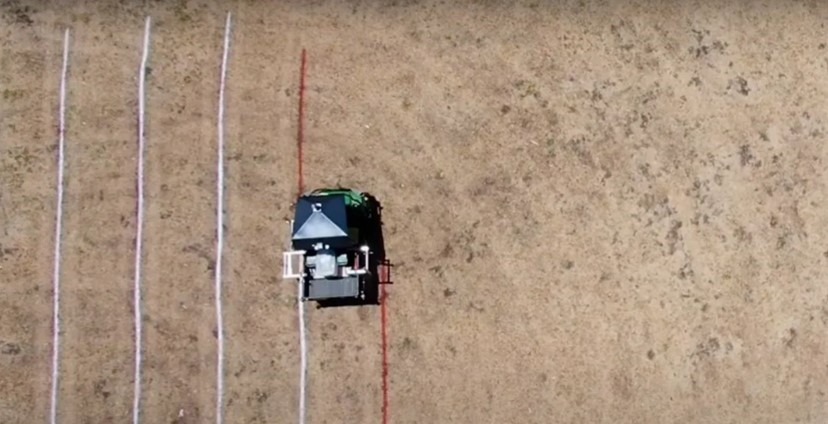
\includegraphics[width=0.45\textwidth]{00 - Images/autonomous_ground_vehicle_for_landmine_clearance.jpg}
  \caption{Autonomous Ground Vehicle for Landmine Clearance \cite{CSIRO2020}}
  \label{fig:autonomous_ground_vehicle_for_landmine_clearance}
\end{wrapfigure}
This is a newly developed mine detection and clearing robot, which uses metal detector sensors to detect mines and could be fitted with a powerful torch that can incinerate mines. We selected this robot because of its ability to collaborate between multiple robots of the same type and the ability to visualize cleared areas. The robot, which is said to approximately be the size of a golf cart, is developed by CSIRO, Data61, and Molten Labs. The robot is fully autonomous and is intended to work together with multiple robots of the same kind. These robots can attach to each other, which also makes them able to drag a malfunctioned robot out of the contaminated area. Furthermore, it allows for quicker mine-clearing when multiple robots are working together. This robot uses a spray-painting system to physically mark the ground that visually shows the areas which have been cleared of mines \cite{CSIRO2020}. It however is a big machine and it could be a troublesome endeavor to deploy multiple robots in a remote area.


\subsubsection*{HUMI}

\begin{wrapfigure}{r}{0.5\textwidth}
    \centering
      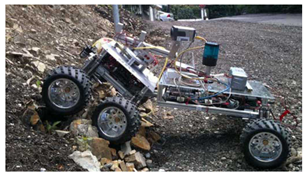
\includegraphics[width=0.45\textwidth]{00 - Images/humi_a_mobile_robot_for_landmine_detection.png}
  \caption{HUMI; A Mobile robot for landmine detection \cite{HUMI2012}}
  \label{fig:humi_a_mobile_robot_for_landmine_detection}
\end{wrapfigure}
This is a six-wheeled semi-autonomous robot used for detecting landmines. We have chosen this robot because of its weight and size. Even though this robot is only a prototype, a demining robot which is based on the prototype HUMI, has been set into full-scale production. HUMI is a light-weight (24,4 kg) demining robot made to be cost-effective. This means that the robot uses cheap available technology such as a landmine detector and its controller. The robot relies heavily on being small, cheap, and easy to use. Its shortcomings are that it is not fully autonomous, only relies on a single metal detector, and that the perception sensors were not available at a reasonable price when it was made \cite{HUMI2012}.

\newpage

\subsubsection*{ClearPath Husky}

\begin{wrapfigure}{r}{0.5\textwidth}
    \centering
      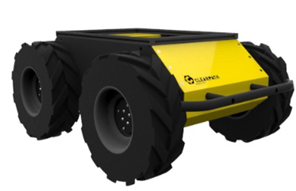
\includegraphics[width=0.45\textwidth]{00 - Images/husky_unmanned_ground_vehicle_robot.png}
  \caption{Husky: Unmanned Ground Vehicle-Robot \cite{ClearPath2020}}
  \label{fig:husky_unmanned_ground_vehicle_robot}
\end{wrapfigure}
This robot is a four-wheeled all-terrain robot. We included this one because of the modularity it provides. This is the main advantage of it. While not specifically designed for demining, ClearPath offers a broad variety of packages to the robot, which can allow the robot to do a multiple of different tasks. The manipulator package is the most ideal package for a demining purpose, this pack-age includes a robotic arm. Of course, this should be in a combination with a metal detector and/or other types of detectors \cite{ClearPath2020}. This was done in the HRATC 2015 competition, which is a community demining competition, in which the goal is to create the best search and mapping algorithm \cite{HRATC2015}. The Husky provides a great traverse ability and can carry a high payload, even in rough terrains. The Husky is priced somewhere in the middle of the price range, as seen in Figure 8. However, it lacks a purposefully designed software for a humanitarian demining operation \cite{ClearPath2020}.\\

An example of the types of sensor which could be used can be seen in Figure \ref{fig:field_robots_for_humanitarian_demining_2014}.

\subsubsection*{SILO-6}

\begin{wrapfigure}{r}{0.5\textwidth}
    \centering
      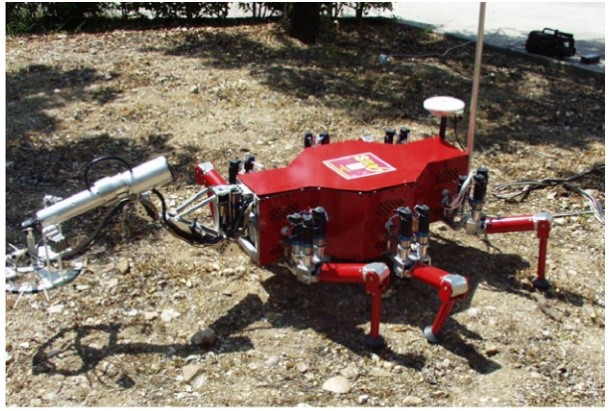
\includegraphics[width=0.45\textwidth]{00 - Images/silo_6_in_action.jpg}
  \caption{SILO-6 In action \cite{6LeggedRobot2007}}
  \label{fig:silo_6_in_action}
\end{wrapfigure}

This robot is also mentioned in Figure \ref{fig:field_robots_for_humanitarian_demining_2014}. It provides a very interesting design, which is very different from the rest of the spectrum. We have selected this because of the six-legged platform which is different from the other examples. This makes it very mobile even in rough terrain and gives a lot of freedom when moving because of the independently moving legs. Six legs have proven to increase stability compared to four legs and are stable in natural terrain which is important when using some sensing technologies. It is fitted with a metal detector but could be getting additional sensors if needed. It is a relatively lightweight (71,34 kg) semi-autonomous robot \cite{6LeggedRobot2007}. This robot could however be hard to replace or do repair work on. Its legs most likely require specially made parts.  ''

\newpage

\subsection{Issues with Current Solutions}

The current solutions have a lot of potential in helping humanitarian demining. Although there is a reason why they are not already hugely implemented in humanitarian work. Every robot has its compromises. It is our intent, to identify and summarize these compromises.

Some of the major issues of the current use of robots, involve oversized robots. Most of them weigh over 70 kg \todo{Strahinja pointed out that it is a MAJOR issue that this part concludes on the payload weight, hence this should be edited troughout the document for the net. weight}. This increases the chance of accidentally activating a mine. HUMI is the only light robot, but this also limits the available space for sensors. But with optimization, and newer technologies available, it should be possible to fit other sensors as well. Robots that weigh hundreds of kilograms and are based on all-terrain vehicles (ATV) or golf carts provide issues regarding transportation. Other robots are limited in the lack of software, and some are limited because of the potential price to repair parts. Most solutions are quite expensive as shown in Figure \ref{fig:field_robots_for_humanitarian_demining_2014} and this cost would properly be an issue for many humanitarian organizations’ budgets. Overall, most of the robots are good solutions, but we propose a solution which also takes these aspects into consideration.